The goal of our research is to develop an automatic way to detect design and requirement \SATD comments. To do so, we first manually classify a large number of comments identifying which ones are \SATD. With the resulting dataset, we train Stanford Classifier to identify design and requirement \SATD (RQ1). Second, we inspect the features used by Stanford Classifier to identify \SATD. These features are words frequently found in comments with technical debt. We present which are the 10 most common words that indicates design and requirement \SATD (RQ2). Then, we investigate how variations in the amount of training data affects the performance of Stanford Classifier classification (RQ3). We detail the motivation, approach and present the results of each of our research questions in the remainder of this section.    

\begin{figure*}[!thb]
  \centering
  \subfigure[Design Debt]{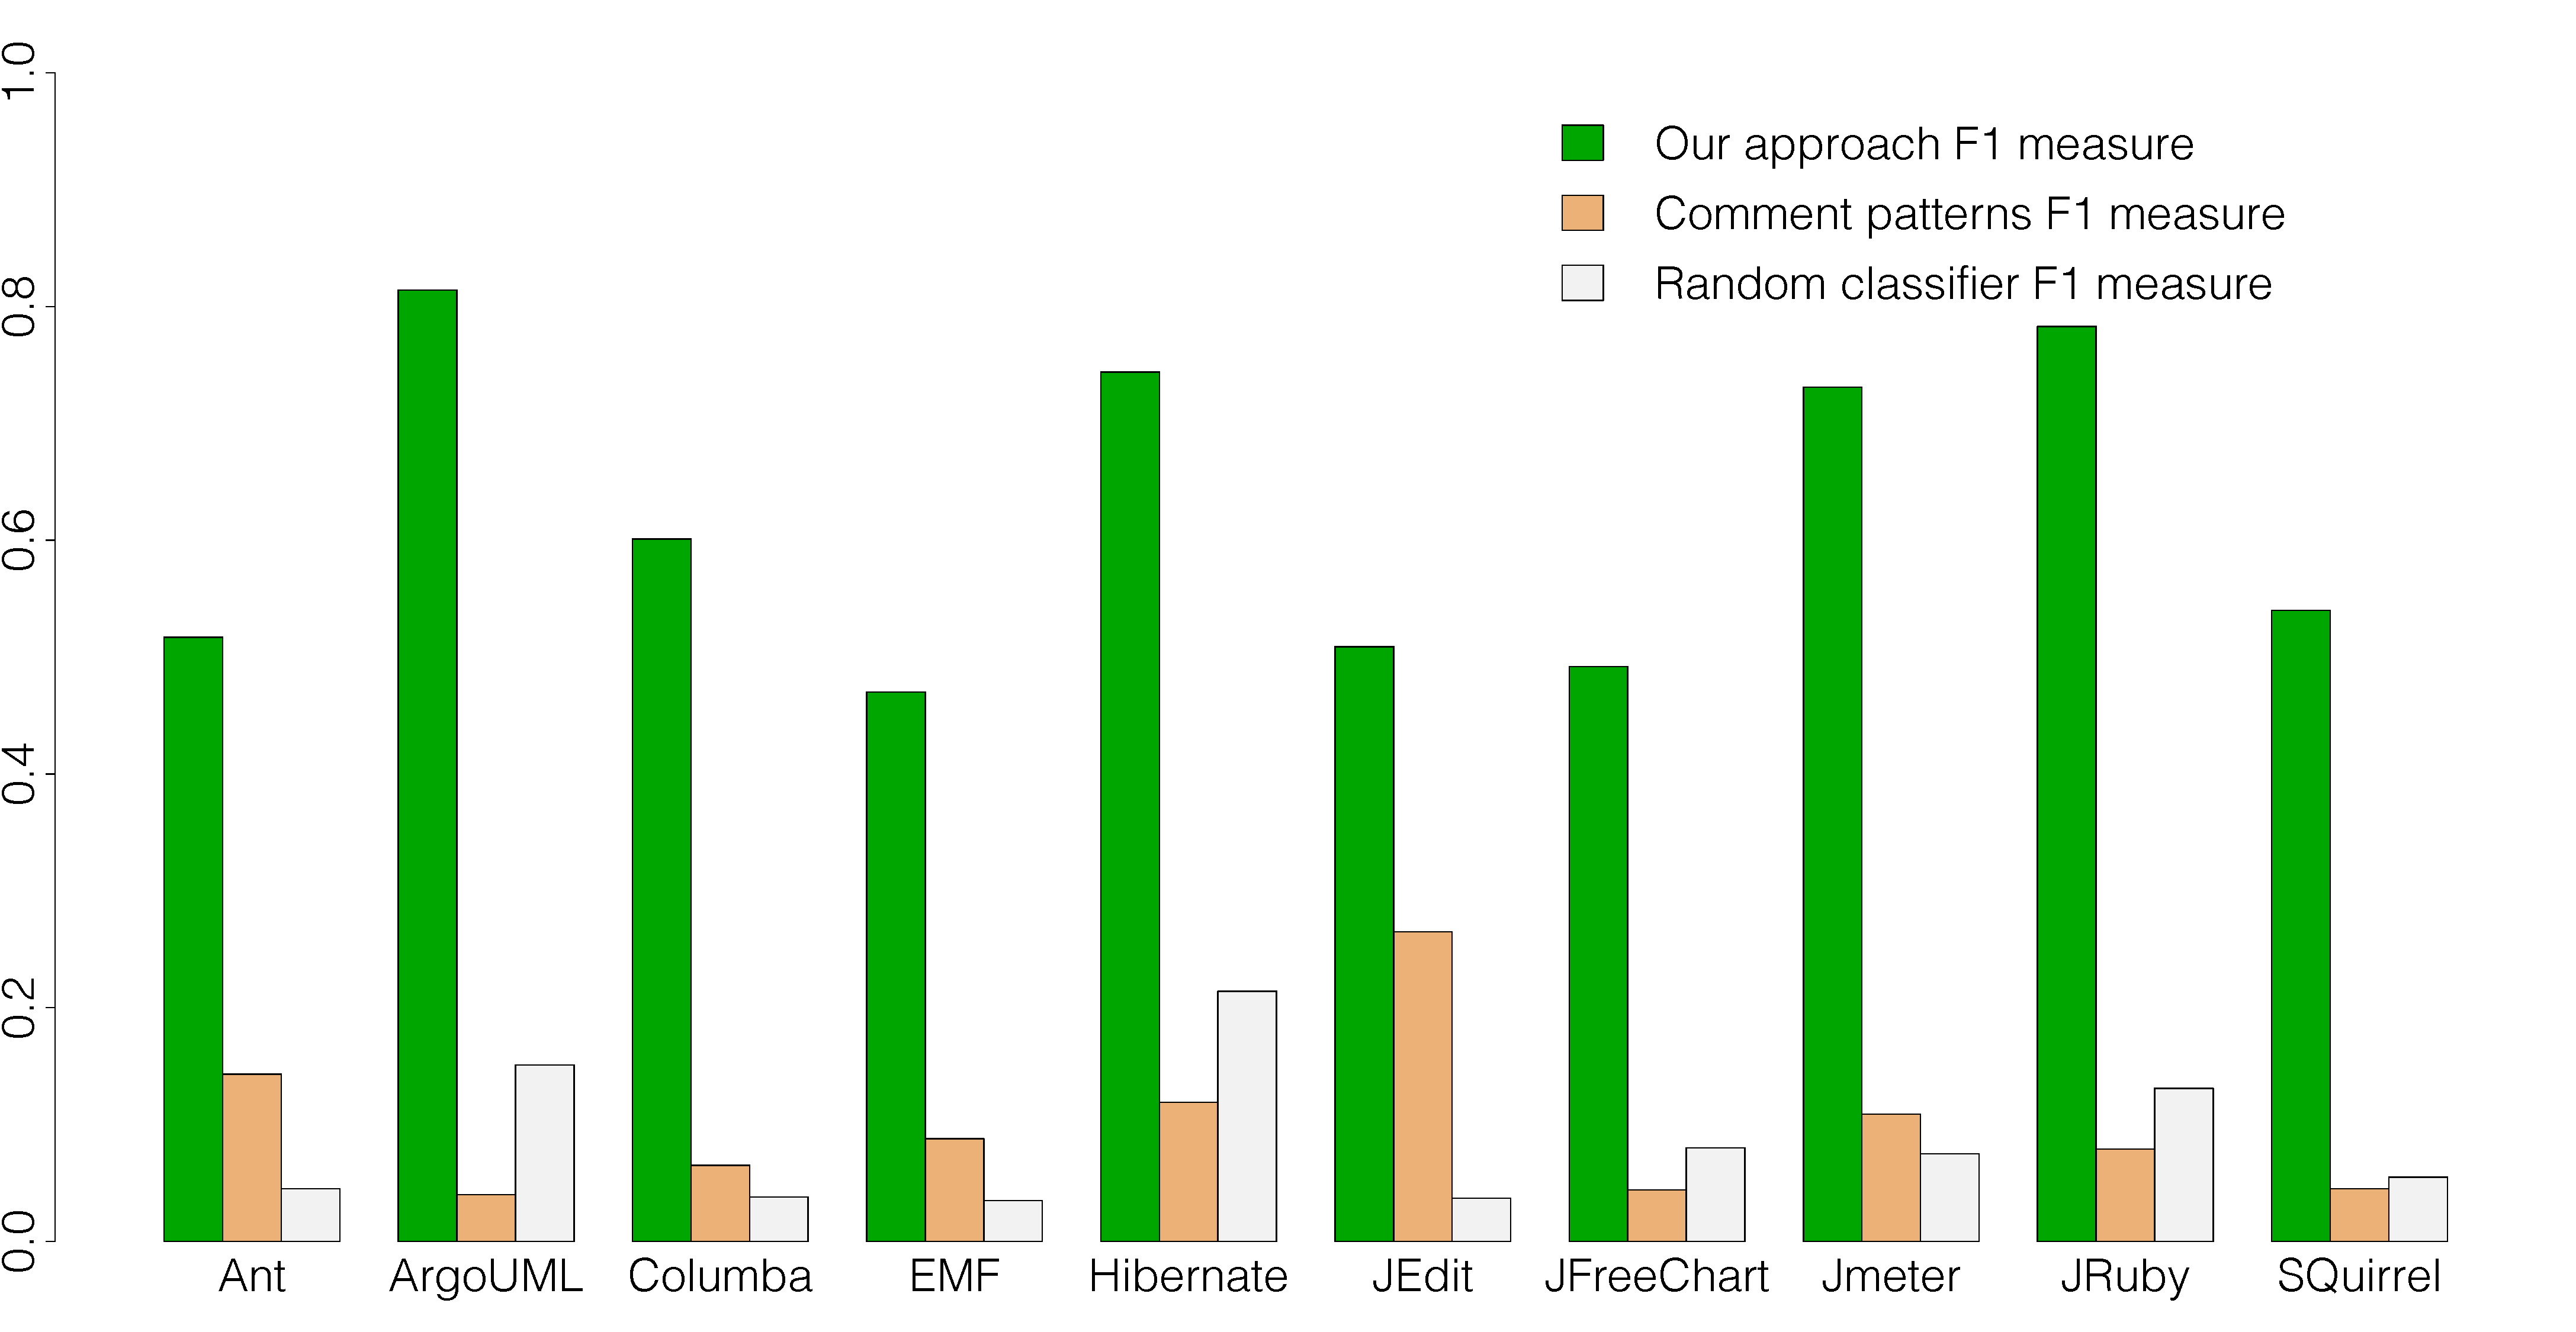
\includegraphics[width=0.48\textwidth]{figures/f1_measure_comparisom_design.pdf}
  \label{fig:f1_measure_comparison_design_debt}}
  \subfigure[Requirement Debt]{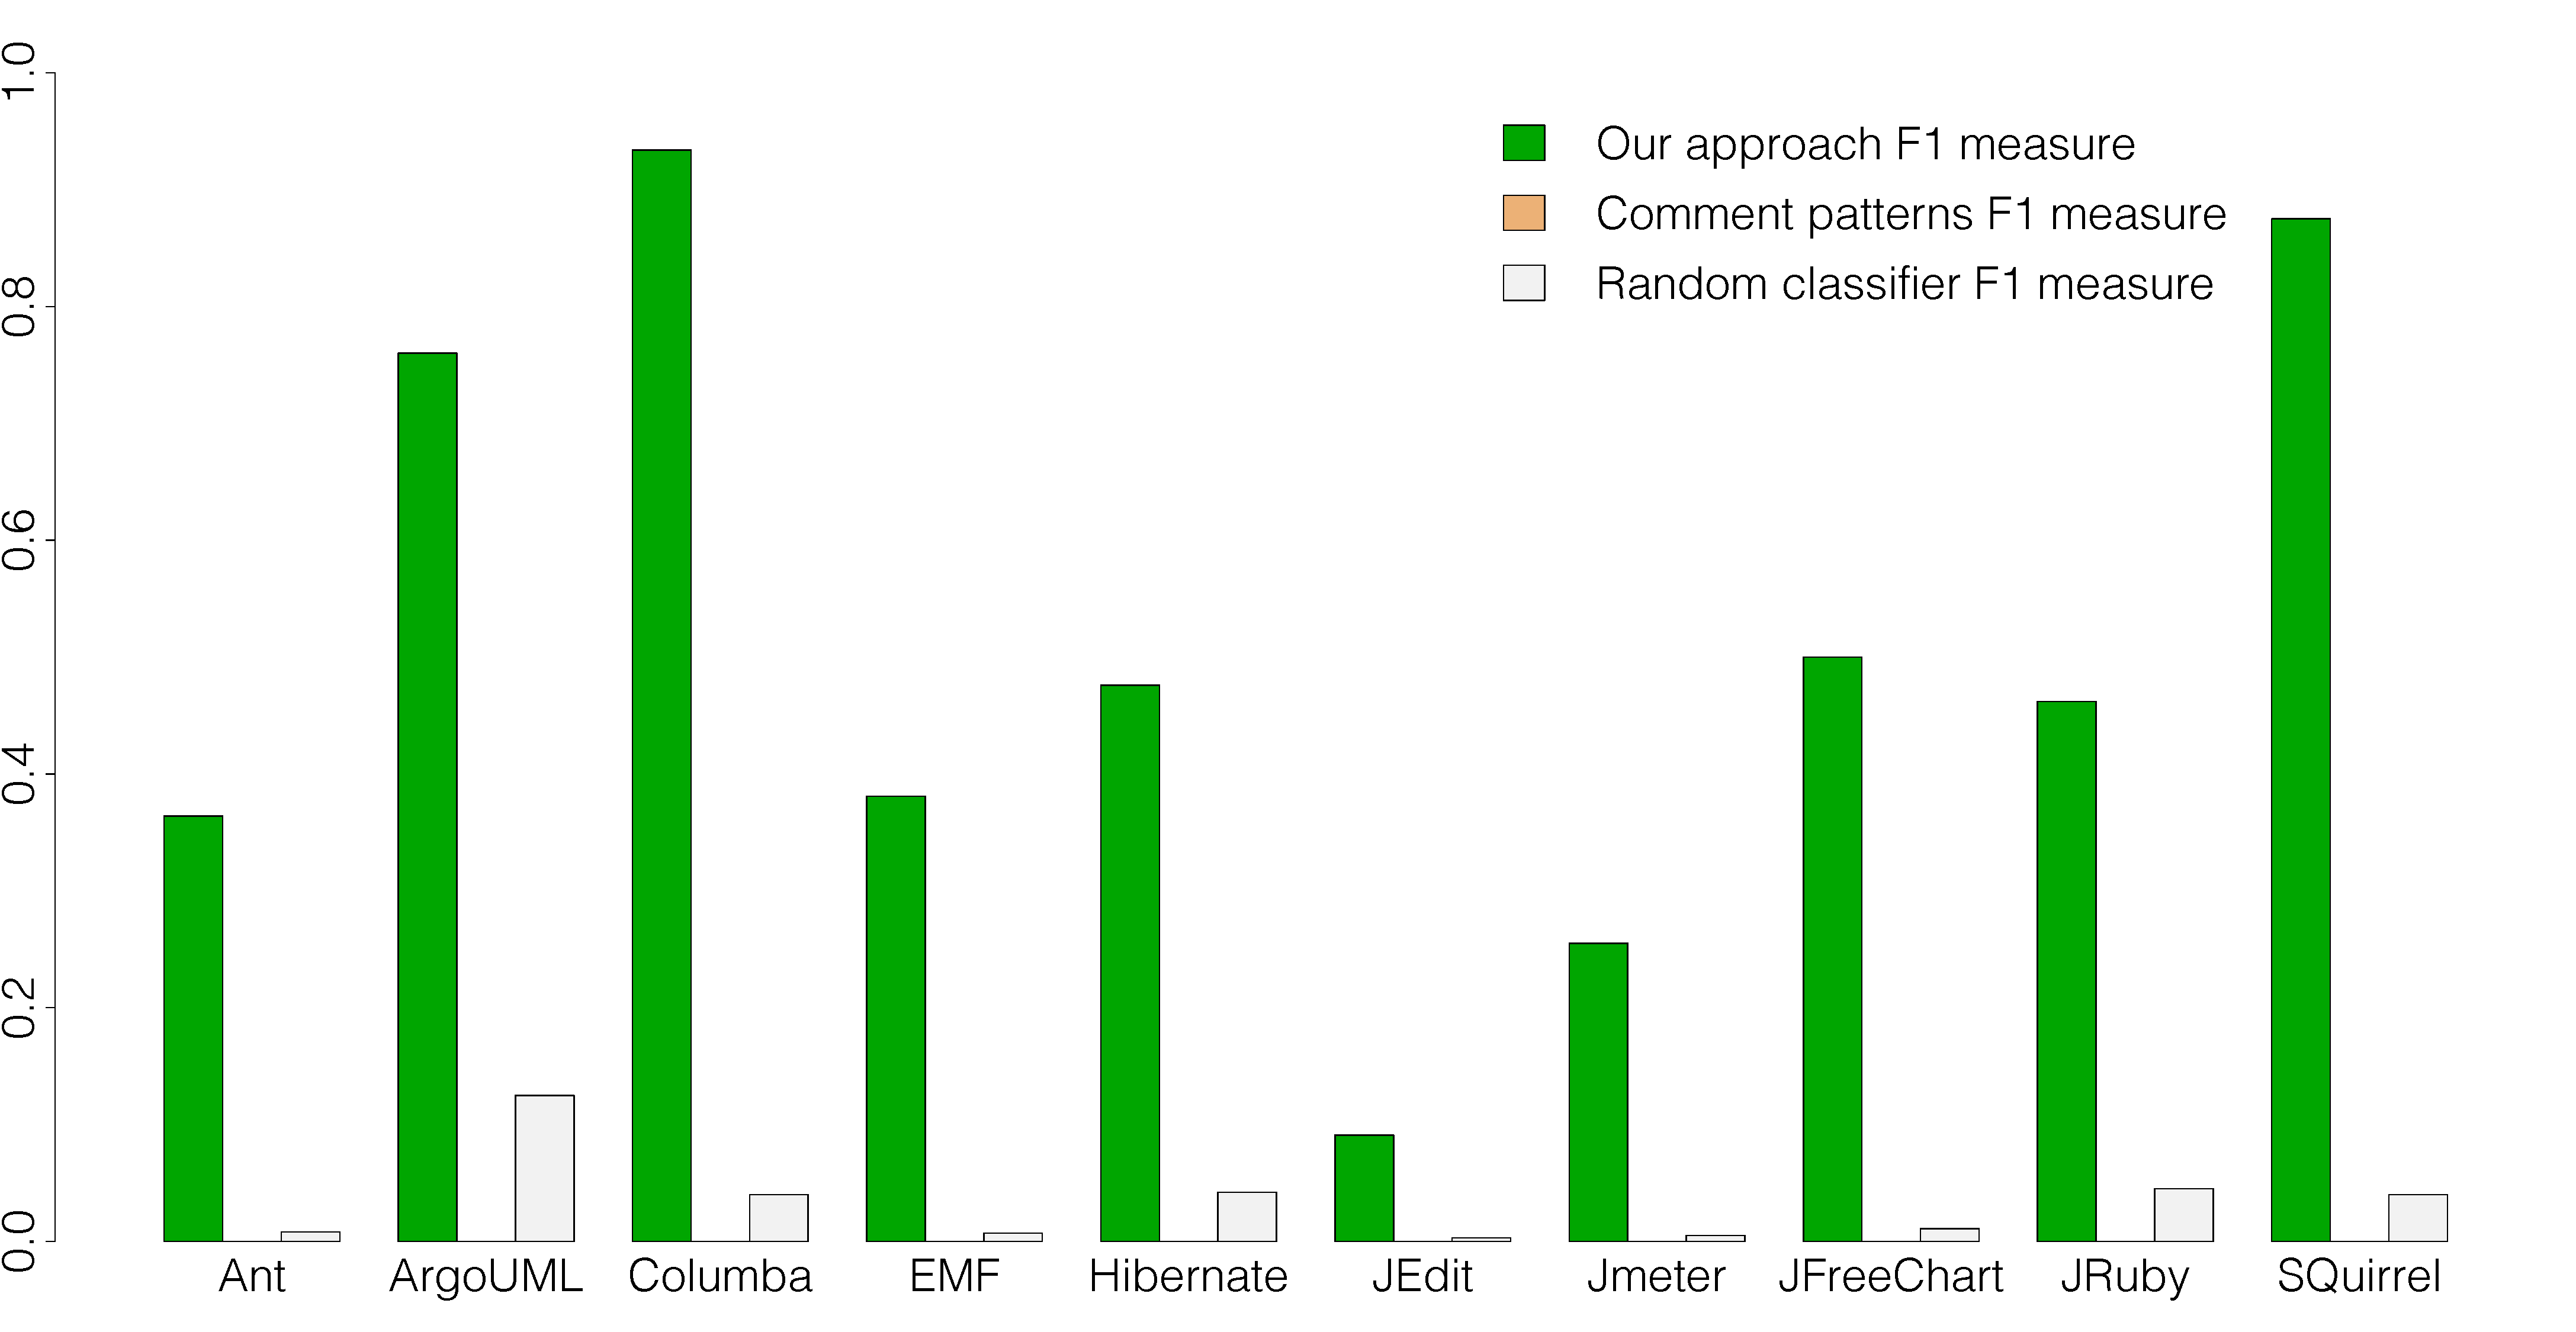
\includegraphics[width=0.48\textwidth]{figures/f1_measure_comparison_requeriment.pdf}
  \label{fig:f1_measure_comparison_requirement_debt}}
  \caption{F1 measure comparison}
\end{figure*}

\begin{table*}[!thb]
    \begin{center}
        \caption{Improvement over the baseline F1 measure for design and requirement debt}
        \label{tbl:improvement_f1measure}
        \begin{tabular}{l| c c c c c c}
        \toprule
        \thead{Project} & \thead{Design Debt \\F1 measure} & \thead{Baseline\\F1 measure} & \thead{Design Debt \\Improvement}& \thead{Requirement Debt \\F1 measure} & \thead{Naive Baseline\\F1 measure}  & \thead{Requirement Debt \\Improvement}\\
        \midrule                                                  
        Ant          &  0.517  & 0.142  &  3.6  x  & 0.364  &  0.008  & 45.5 x  \\
        ArgoUML      &  0.814  & 0.040  &  20.3 x  & 0.760  &  0.005  & 152  x  \\
        Columba      &  0.601  & 0.065  &  9.2  x  & 0.934  &  0.125  & 7.4  x  \\
        EMF          &  0.470  & 0.087  &  5.4  x  & 0.381  &   0.04  & 9.5  x  \\
        Hibernate    &  0.744  & 0.118  &  6.3  x  & 0.476  &  0.007  & 68   x  \\
        JEdit        &  0.509  & 0.264  &  1.9  x  & 0.091  &  0.042  & 2.1  x  \\
        JFreeChart   &  0.492  & 0.044  &  11.1 x  & 0.500  &  0.003  & 166.6 x  \\
        Jmeter       &  0.731  & 0.108  &  6.7  x  & 0.255  &  0.011  & 23.1  x  \\
        JRuby        &  0.783  & 0.078  &  10   x  & 0.462  &  0.045  & 10.2  x  \\
        SQuirrel     &  0.540  & 0.044  &  12.2 x  & 0.875  &   0.04  & 21.8  x  \\
        \bottomrule
        \end{tabular}
    \end{center}    
\end{table*}

\vspace{3mm}
\noindent\rqi
\vspace{3mm}

\noindent \textbf{Motivation:} As shown in previous work \cite{Potdar2014ICSME, Maldonado2015MTD}, \SATD comments can be found in the source code. However, there is not an automatic way to identify these technical debt comments yet. The methods proposed so far heavily relies on manual examination, and there are too little evidence on how well these approaches perform and how applicable they are. We want to determine if natural language processing tools such as Stanford Classifier can help us to surpass these limitations. Stanford Classifier automatically classify comments based on specific linguistic characteristics that developers uses while writing comments. These characteristics are obtained through the training dataset that we created. 

For example, the training dataset can show that the adjective `ugly' is frequently found in \SATD comments. Answering this question is important to help us understand the opportunities and limitations of automatic identification of \SATD comments. 

\vspace{1mm}
\noindent \textbf{Approach:} As described in Section \ref{sec:approach}, we manually classify comments from ten open source projects into one of the following types of \SATD: design debt, defect debt, implementation debt, documentation debt and test debt. However, as shown in our previous work \cite{Maldonado2015MTD}, the most frequent \SATD comments are design and implementation debt respectively. Therefore, we focuses our attention in the identification of these two \SATD types. 

We design our case study to test how well the Stanford Classifier identifies \SATD comments when trained with our manually created dataset. Our training dataset contains comments with and without \SATD, and each comment contains its own classification (i.e., without technical debt, design debt or requirement debt). Then, we add to the training dataset all comments classified as without technical debt and the comments classified as the specific type of \SATD that we want to predict. We use comments from 9 out of 10 projects that we analyzed to create the training dataset. The comments from the remaining project is used to evaluate the classification performed by Stanford Classifier.

For example, if we want to classify the design \SATD comments in Ant project we create the training dataset using all design \SATD comments and the all comments classified as without technical debt from the other nine projects. Then, we use the comments of Ant to create the test dataset. 

The next step is to execute the Stanford Classifier. Based on the training dataset Stanford Classifier will classify each comment in the test dataset. The resulting classification is compared with the manual classification provided in the test dataset and evaluated. If a comment in the test dataset has the same classification that the classification suggested by Stanford Classifier we will have a true positive or a true negative. True positives are the cases that Stanford Classifier identified correctly \SATD comments, and true negatives when comments without technical debt are classified as so. 

Similarly, when the classification provided by the tool diverges from the classification provided in the test dataset we have false positives or false negatives. False positives are comments classified as being \SATD when they are not, and false negatives are comments classified as without technical debt despite the fact that the classification in the test dataset says the contrary.

Asserting the number of true positives (tp), true negatives (tn), false positives (fp) and false negatives (fn) we can evaluate the performance of the Stanford Classifier in terms of Precision (i.e., $\frac{tp}{tp + fp}$), Recall (i.e., $\frac{tp}{tp + fn}$) and F1 measure (i.e., $2 \times \frac{P \times R}{P + R}$).

To determine how effective Stanford Classifier classification are we compare its F1 measure with the F1 measure of two other approaches. The first approach is the current state-of-the-art in detection of \SATD comments devised by Potdar and Shihab ~\cite{Potdar2014ICSME}. This approach uses 62 comment patterns (i.e., keywords) that were noticed as recurrent in \SATD comments during the manual inspection of 101,762 comments. 

The second approach is a naive baseline which depends on the distribution of the data. Self-admitted technical debt comments are much more uncommon than comments without technical debt. The naive baseline is meant to show this discrepancy in the data distribution. For example, Ant has 4,140 comments, of those, only 95 comments are design \SATD. The chance to randomly find a design \SATD comment is of 0.023 (i.e., $\frac{95}{4140}$). 

Lastly, for each project we obtained the comment patterns baseline and the naive baseline. Then, we store all results in a database to perform our analysis. 

\vspace{1mm}

\noindent \textbf{Results:} We find that the Stanford Classifier classification greatly outperforms the comment patterns baseline and the naive baseline as well. Figure \ref{fig:f1_measure_comparison_design_debt} presents the comparison between the Stanford Classifier F1 measure, the comment patterns baseline F1 measure and the naive baseline F1 measure while identifying design \SATD. We choose to use the F1 measure to compare the performance between the approaches as this measurement provides the harmonic mean of precision and recall.

It is important to notice that each one of the selected baselines for comparison has one strong point. The comment patterns approach has a high precision, but it lacks recall, i.e., this approach points correctly to \SATD comments, but as the approach depends on keywords, it identifies a very small set of all the \SATD comments in the project. The less sophisticated naive baseline provides a high recall because we try to classify comments between two categories (i.e with or without technical debt), meaning a 50\% chance to randomly get one of the two classifications. 

For all the projects, the F1 measure achieved by Stanford Classifier is higher than the other baselines F1 measures. The highest F1 measure obtained for design debt was in ArgoUML with a value of 0.814. On the other hand, the lowest F1 measure obtained was in EMF with a value of 0.470. On average, the obtained F1 measure was 0.620. In comparison, the average F1 measure obtained using comment patterns was of 0.099, and the naive baseline F1 measure 0.086. Consequently, our approach to identify design \SATD outperforms, in average, 6 times the state-of-the-art approach and 7 times the naive baseline. The third column of Table \ref{tbl:improvement_f1measure} shows the improvement of our approach over the comment patterns baseline for each project. 
 
Similarly, Figure \ref{fig:f1_measure_comparison_requirement_debt} shows the comparison between the three F1 measures while identifying requirement \SATD.

We find that the comment patterns approach is not an appropriate approach for identifying requeriment \SATD, since it was not able to identify any of the requirement \SATD in our analyzed projects. Therefore, we use the naive baseline to comparare with our results.

For all projects, the F1 measure obtained by our approach greatly surpass the naive baseline. Our highest F1 measure was obtained for Columba project with 0.934, and the lowest value was of 0.091 on JEdit. Although there was a big fluctuation between the maximum and minimum value obtained our average F1 measure was of 0.510. 

Despite the fact that this number is slightly lower than the average obtained while  identifying design debt, the quantity of requirement \SATD comments that are present in the projects are very low, which makes its classification more difficult. For example, JEdit has 14 requirement \SATD comments distributed over a total of 10,109 comments (i.e, requirement debt comments plus without \SATD comments). Nevertheless, our approach can identify \SATD even in this unbalanced dataset as we still outperform the naive baseline F1 measured by 30 times, i.e., the naive baseline F1 measure was of 0.003 for JEdit. 

The seventh column of Table \ref{tbl:improvement_f1measure} shows the improvement of our approach over the naive baseline. For SQuirrel the F1 measure was of 0.875 whereas the naive baseline F1 measure was of 0.04, which means that there was an improvement of 21.8 times in the identification of requirement \SATD comments using our approach. 

\conclusionbox{We find that the Stanford Classifier, is more effective identifying \SATD comments than the current state-of-art approach. We achieved an average F1 measure of 0.62 while identifying design debt and an average of 0.51 while classifying requirement debt.}

\vspace{3mm}
\noindent\rqii
\vspace{3mm}

\noindent \textbf{Motivation:} After asserting the efficiency of Stanford Classifier identifying \SATD comments we want to better understand what words developers use when indicating \SATD comments. Answering this question will provide insightful information that can guide future research direction, broaden our understanding on \SATD and also help us to detect it.     

\vspace{1mm}
\noindent \textbf{Approach:} As mentioned before, we use the Stanford Classifier to identify \SATD comments, and the first part of the identification process is to generate the features (i.e., words) that will be used to classify the comments. These features, are fragments of data that possesses a class (i.e., design debt, requirement debt or without technical debt) and a weight. These features are extracted from the comments in the training dataset, and then applied to the test dataset where they are combined to reach a vote. That is, every feature that is satisfied by the comment being classified (i.e., matched) will be used to predict the class for the comment. The vote is given to the class with highest weight. 

For example, we have two design debt features: `hack' and `dirty' with weight of 5.3 and 3.2 respectively, and one without technical debt feature: `ignored' with weight of 4.1. When classifying the following comment ``this is a dirty hack and should not be ignored'', all features would have been matched, and the vote decision would be: design debt weight = 8.5 (i.e., feature `hack' weight plus feature `dirty' weight) and without technical debt weight = 4.1 resulting in a comment classified as design debt.

For each project analyzed we collect the features used to predict the \SATD comments. These features are provided by Stanford Classifier as output and stored in a text file. The features are written in the file based on the weight that it has, ordered by highest weight to the lowest weight meaning more relevant features to less relevant features respectively. Based on these files, we rank the words calculating the average ranking position of the analyzed feature across the ten different files. 

We determined the top 10 features (i.e, most relevant based on the weight) for design and requirement \SATD comments.

\vspace{1mm}
\noindent \textbf{Results:} Table \ref{tbl:top_ten_features} shows the top 10 features for the identification of \SATD in the ten studied projects ordered by relevance. In the first column we present the ranking of the word. In the second column we list the features used in the identification of design \SATD, and the third column is the list of features used to identify requirement \SATD.

\begin{table}[!thb]
    \begin{center}
        \caption{Top ten features for Self-Admitted Technical Debt}
        \label{tbl:top_ten_features}
        \begin{tabular}{l| l l }
        \toprule
        \thead{Order} & \thead{Design\\Debt} & \thead{Requirement\\Debt}  \\
        \midrule
         1  & hack       &   todo              \\
         2  & workaround &   needed            \\
         3  & yuck!      &   implementation    \\
         4  & kludge     &   fixme             \\
         5  & stupidity  &   xxx               \\
         6  & needed?    &   ends?             \\
         7  & columns?   &   convention        \\
         8  & unused?    &   configurable      \\
         9  & wtf?       &   apparently        \\
         10 & todo       &   auto-generated    \\
        \bottomrule
        \end{tabular}
    \end{center}    
\end{table}

It is possible that the same feature is used to classify design debt and requirement debt. However, the weight of this feature can be different accordingly with the type being classified. As we can see in Table \ref{tbl:top_ten_features}, `fixme' and `todo' appears in both columns although they have a higher ranking when classifying requirement debt than design debt. 

In spite of the fact that features with higher weights will have more impact during the classification, the final vote is given based on the combined weight of all matching features. In average, the number of features to classify design debt were 6,196 whereas for requirement debt they were 2,889. This shows why our recall is much better than Potdar and Shihab's ~\cite{Potdar2014ICSME}. 

\conclusionbox{We find that the most common words indicating \SATD comments are: `hack', `workaround', `yuck!', `kludge', `stupidity', `needed', `columns?', `unsed?', `wtf?', `todo', `implementation', `fixme', `xxx', `ends?', `convention', `configurable', `apparently' and `auto-generated'.}

\vspace{3mm}
\noindent\rqiii
\vspace{3mm}

\noindent \textbf{Motivation:} We shown that we can effectively identify \SATD comments. However, the classification of \SATD comments depends on the training dataset that was manually created. But, how much training data do we need to classify these comments? If we need a high number of comments to create our training dataset our approach will be more difficult to be extended and applied in different contexts. In the other hand, if a small dataset can be used to identify \SATD comments this approach can be applied to applications other than Java and even to comments written in different idioms. 

\vspace{1mm}
\noindent \textbf{Approach:} We executed the classification process several times with an increasing number of comments being added to the training dataset while collecting the results to analyze the changes between each iteration.

We first select a project that will be classified by the Stanford Classifier.

Second, with one of the remainder projects, we select all \SATD comments (i.e., design or requirement debt accordingly with what we want to classify), and all comments without technical debt as well. These comments are added to the training dataset and fed into the Standford Classifier. Then, the results of the classification are collected and stored to analysis.

Third, the comments of other project is added to the training dataset and the results of the classification are collected once more. The order that projects are added to the training dataset is not random. We add first projects which has more \SATD comments of the specific type that we are trying to identify. We cycle through the above steps until we had added the comments of all nine projects to the training dataset.

Fourth, we select another project to be classified by the Stanford Classifier, and we repeat this process until we have analyzed all our projects.
 
To determine how much data is necessary to effectively identify \SATD comments we analyze the iteration with highest F1 measure and the number of comments used in the training dataset to achieve this mark. Based on the maximum F1 measure we calculate how close the others iterations were from achieving the same value.

For example, if the maximum F1 measure was 0.85 achieved in the 8th iteration, and during the 4th iteration we had a F1 measure of 0.80 we say that 94\% of the maximum F1 measure was achieved in the 4th iteration. Once the percentage of the maximum F1 measure is calculated for all iterations we analyze the quantity of comments used in the training dataset by them.

\begin{figure}[t]
  \centering
  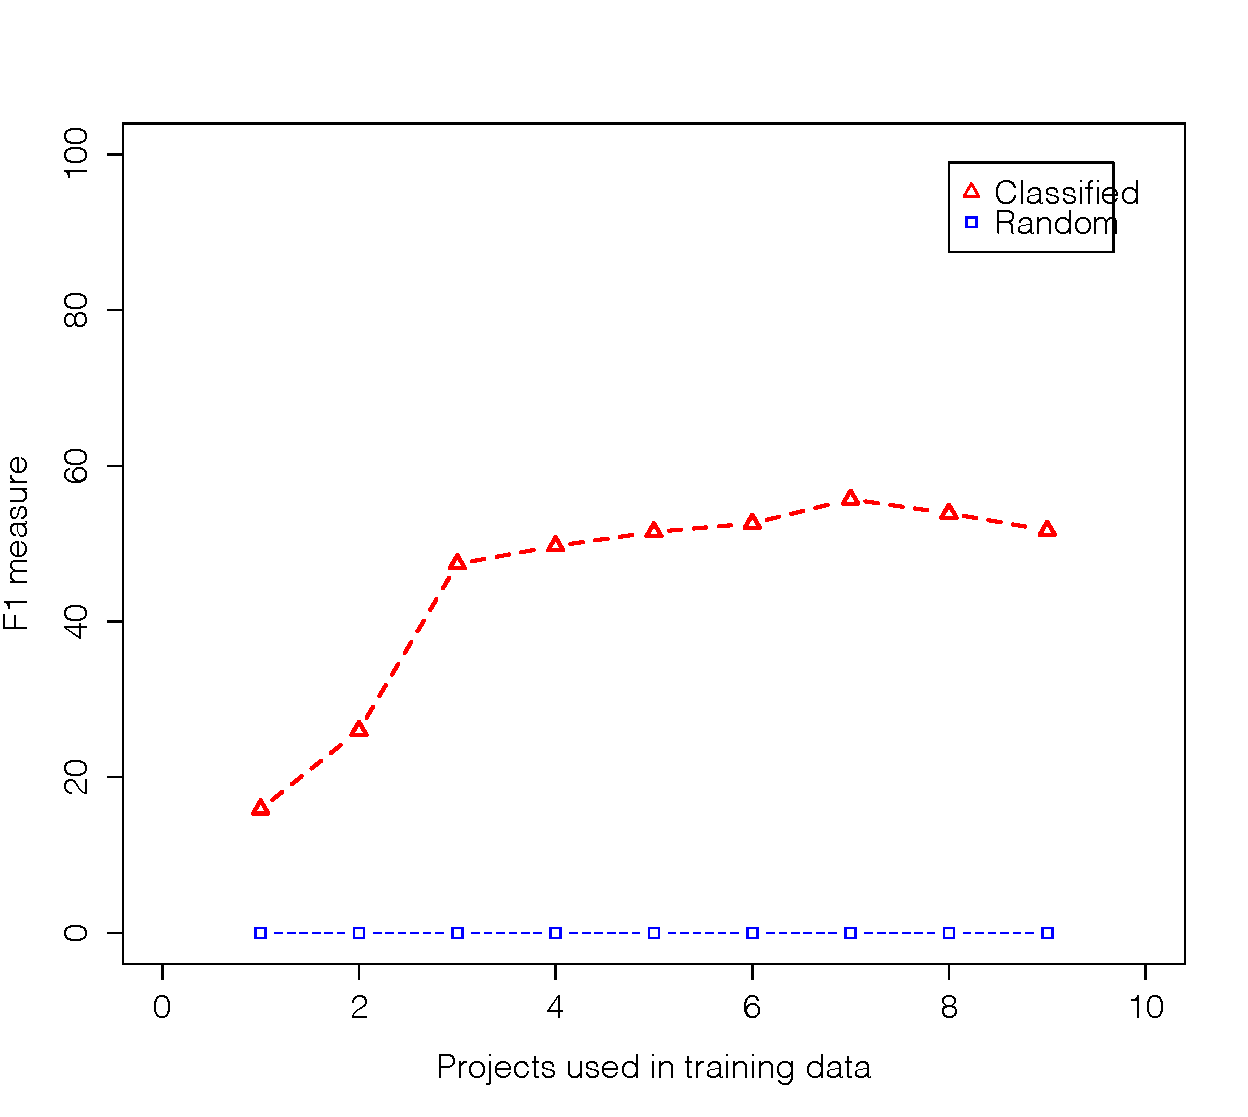
\includegraphics[width = 0.48\textwidth]{figures/design_ant.pdf}
  \vspace{-3mm}
  \caption{Ant Design Debt classification}
  \label{fig:design_ant_result}
\end{figure}

\begin{figure}[t]
  \centering
  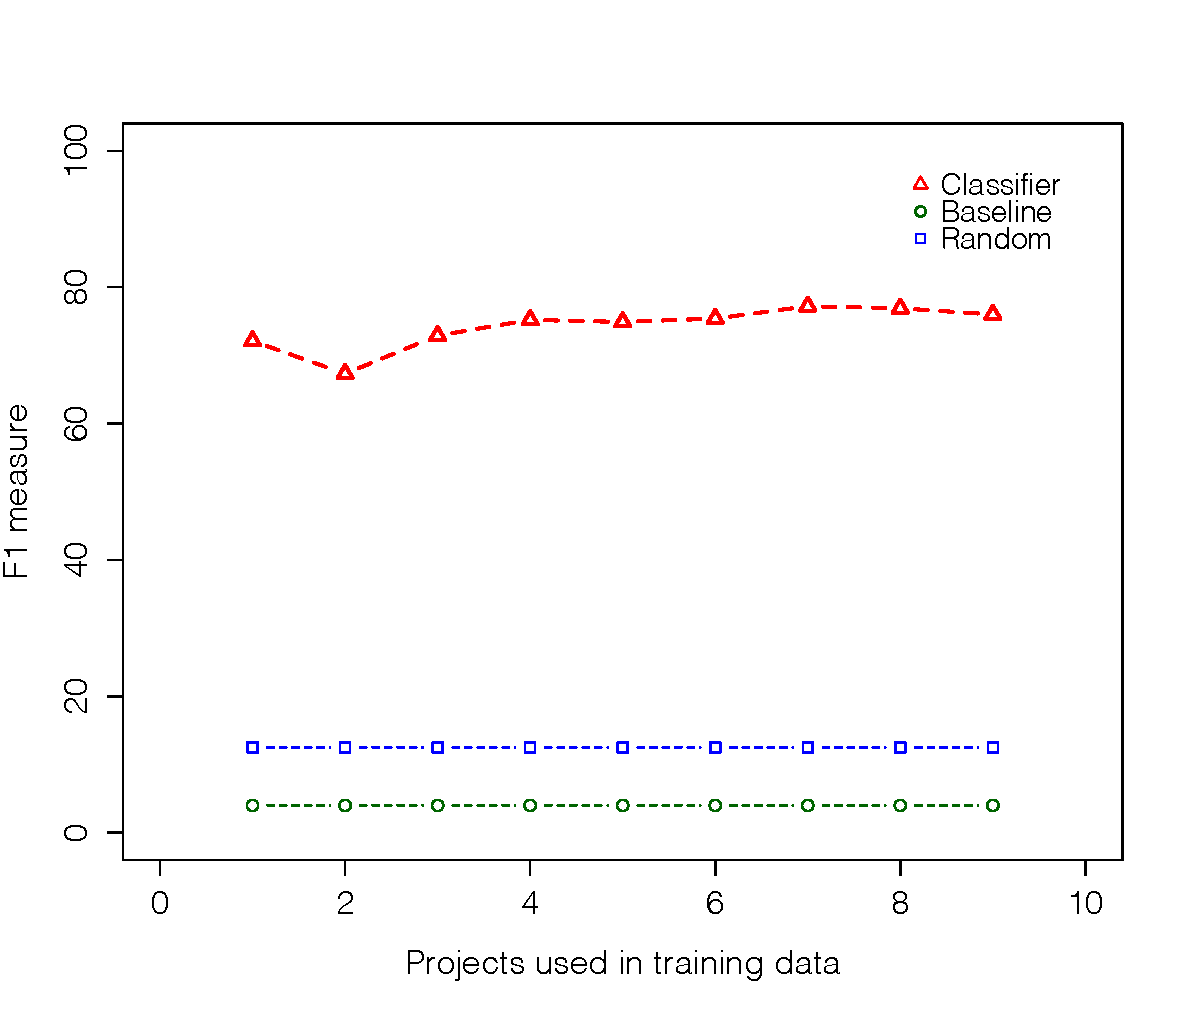
\includegraphics[width = 0.48\textwidth]{figures/implementation_argo.pdf}
  \vspace{-3mm}
  \caption{ArgoUml Requirement Debt classification}
  \label{fig:implementation_argo_result}
\end{figure}

\vspace{1mm}
\noindent \textbf{Results:} Intuitively we expect that the performance of the classifier would improve with each iteration as more comments are being added to the training dataset. However, we find that this is not what always happens, and that the addition of more comments can decrease the performance of the classifier in given scenarios. One of the reasons for this is that the weight of features is given through empirical probability, and consequently features that appears more will have a higher weight. Although this is an effective process for the majority of cases that we studied, it can be misleading when classifying comments that has different context from the comments found in the training dataset. 

Therefore, we determined which iteration has the highest performance for each project. We called this iteration as the maximum F1 measure. To know how close the other iterations were from reaching the maximum performance we use the iteration F1 measure value to calculate the percentage of the maximum F1 measure that it represents. We calculate these values for design and requirement debt separately.

\vspace{1mm}
\noindent \textbf{Design debt:} We find that the F1 measure improves significantly in the first three iterations and, after that, the improvement rate is more steady. Figure \ref{fig:design_ant_result} shows this behavior using Ant as an example. For the sake of space we only provide the figure of one analyzed project, but we performed this analysis for all ten projects and Ant is a good representation of our results. 

The three highest values of the F1 measure in Figure \ref{fig:design_ant_result} are: 0.526, 0.539 and 0.557 obtained during the 6th, 8th and the 7th iteration respectively.

We notice that in the 3rd iteration the F1 measure was 0.474, and the maximum F1 measure achieved for the project (i.e., 7th iteration) was 0.557. The F1 measure achieved in the 3rd iteration represents 85\% of the maximum F1 measure achieved in the 7th iteration, and this percentage was reached using 1,499 comments (i.e., from 3 projects) whereas the maximum F1 measure used 2,404 comments (i.e., from 7 projects) in the training dataset. Therefore, for Ant we could achieve 85\% of the maximum result using only 62\% of the comments. We argue that the third iteration provides a good tradeoff between prediction performance and number of comments used to create the training dataset.

Because the collected results are slightly different from each other, we analyzed the iterations individually to determine which iteration has the best performance across all projects. To measure that, we calculate the average percentage of the maximum F1 measure for each iteration. For example, we take the average percentage of the maximum F1 measure achieved during the 1st iteration for all projects, then we calculate the same value for all 2nd iterations and so on. We find that, in average, the best performance is achieved during the 8th iteration.

At the 8th iteration the average of the maximum F1 measure is of 96.57\% using on average 2,353 comments to create the training dataset. In comparison, the 9th iteration have an average of the maximum F1 measure of 95.99\% which is slightly lower than the average obtained in the 8th iteration, and uses more comments in the training dataset (i.e., 2,432). As mentioned before, the addition of more comments not necessary implies in more performance.

Table \ref{tbl:design_iteration_performance} shows the average percentage of the maximum F1 measure for each iteration. The first column shows the iteration number. The second column shows the average percentage of the maximum F1 measure achieved for each iteration. The third column presents the delta interval of the average percentage of the maximum F1 measure between one iteration and another. The fourth column shows the average of comments used in the training dataset of that specific iteration.

We found that, the third iteration presents an average of the maximum F1 measure of 92.47\%, and uses 1,444 comments in average in the training dataset. This means using only 59.37\% of the total comments classified in this study (i.e., 2,432 design \SATD). 

\vspace{1mm}
\noindent \textbf{Requirement debt:} We find that although there is variation in the F1 measure value during the first 3 iterations they are not so preeminent as the variation found in design \SATD analysis. The F1 measure in requirement \SATD tend to be more constant through the iterations, and the first iteration has already a high percentage of the maximum F1 measured achieved for each project. This shows that the way the developers indicate requirement debt does not vary between different application domains as much as in design debt. This uniformity in requirement \SATD comments allows a good classification even with a small number of comments in the training dataset.  

Figure \ref{fig:implementation_argo_result} shows the performance of the F1 measure over the iterations in ArgoUml. The highest values of the F1 measure shown in Figure \ref{fig:implementation_argo_result} are in order execution: 0.772 (7th), 0.769 (8th) and 0.760 (9th).

ArgoUML has F1 measure of 0.721 during the 1st iteration, 0.729 in the third iteration and 0.772 in the seventh iteration which was the highest F1 measure achieved. The improvement in the F1 measure between the 1st and 3rd iteration is very low as it is between the 4th and the 6th iteration. In the 1st iteration the classifier was trained with 150 requirement \SATD comments, which means 27\% of the comments that where used in the 9th iteration. A reduction of 73\% of the necessary training data to achieve almost the same result in terms of F1 measure in this case. 

We also analyzed the average percentage of the maximum F1 measure between all iterations across the projects. The 7th iteration was the one with the highest average percentage of the maximum F1 measure achieving a value of 89.89\%. In the 7th iteration an average of 1,055 requirement \SATD comments were used in the training dataset representing 97\% of all requirement \SATD comments that we classified during this study.

We find that the 1st iteration has a hight average of percentage of the maximum F1 across all projects (i.e., 83\%). Although this percentage still lower than the achieved at the 7th iteration (i.e., 88\%), the training dataset of the 1st iteration sized, on average, 601 \SATD comments. This means a reduction of 44\% in the necessary amount of comments to create an effective training dataset to classify requirement \SATD comments. Table \ref{tbl:requirement_iteration_performance} shows the average maximum F1 measure, the delta interval of the average maximum F1 measure between each iteration and the average number of comments used to create the training dataset. 

\begin{table}[!thb]
    \begin{center}
        \caption{Average maximum F1 measure for Design Debt  for all projects}
        \label{tbl:design_iteration_performance}
        \begin{tabular}{l| c c c}
        \toprule
        \thead{Iteration\\Number} & \thead{Average\%\\of maximum\\F1 measure} & \thead{$\Delta$\\between\\iterations} & \thead{Average\\comments} \\
        \midrule
         1  &  0.718 &  -      & 756   \\  
         2  &  0.856 &  0.138  & 1,106 \\  
         3  &  0.924 &  0.068  & 1,444 \\  
         4  &  0.912 & -0.012  & 1,717 \\  
         5  &  0.927 &  0.015  & 1,919 \\  
         6  &  0.930 &  0.003  & 2,108 \\  
         7  &  0.963 &  0.033  & 2,251 \\  
         8  &  0.965 &  0.002  & 2,353 \\  
         9  &  0.959 & -0.006  & 2,432 \\  
        \bottomrule
        \end{tabular}
    \end{center}    
\end{table}

\begin{table}[!thb]
	\begin{center}
		\caption{Average maximum F1 measure for Requirement Debt for all projects}
		\label{tbl:requirement_iteration_performance}
		\begin{tabular}{l| c c c}
			\toprule
			\thead{Iteration\\Number} & \thead{Average\%\\of maximum\\F1 measure} & \thead{$\Delta$\\between\\iterations} & \thead{Average\\comments} \\
			\midrule
			1  &  0.862 &   -      &  601   \\  
            2  &  0.834 & -0.028   &  748   \\
            3  &  0.838 &  0.004   &  876   \\  
            4  &  0.834 & -0.004   &  970   \\
            5  &  0.823 & -0.011   &  1,014  \\
            6  &  0.832 &  0.009   &  1,037  \\
			7  &  0.898 &  0.066   &  1,055  \\  
            8  &  0.885 & -0.013   &  1,071  \\  
            9  &  0.873 & -0.012   &  1,085  \\  
			\bottomrule
		\end{tabular}
	\end{center}    
\end{table}

It is important to notice that, this results shows that it is possible to identify \SATD with a lower number of comments. Using a lower number of comments to create the training dataset makes the approach more applicable as the number of \SATD comments is rather scarce.    

\conclusionbox{We find that the design \SATD comments can be classified effectively using a training dataset of 1,444 comments. Similarly, requirement \SATD can be classified with as many as 601 comments of this type.}